\clearpage
\section{Ellipsoidal Objects}
\label{sect:EllipsoidalObjects}
\begin{figure}[htb]
\begin{center}
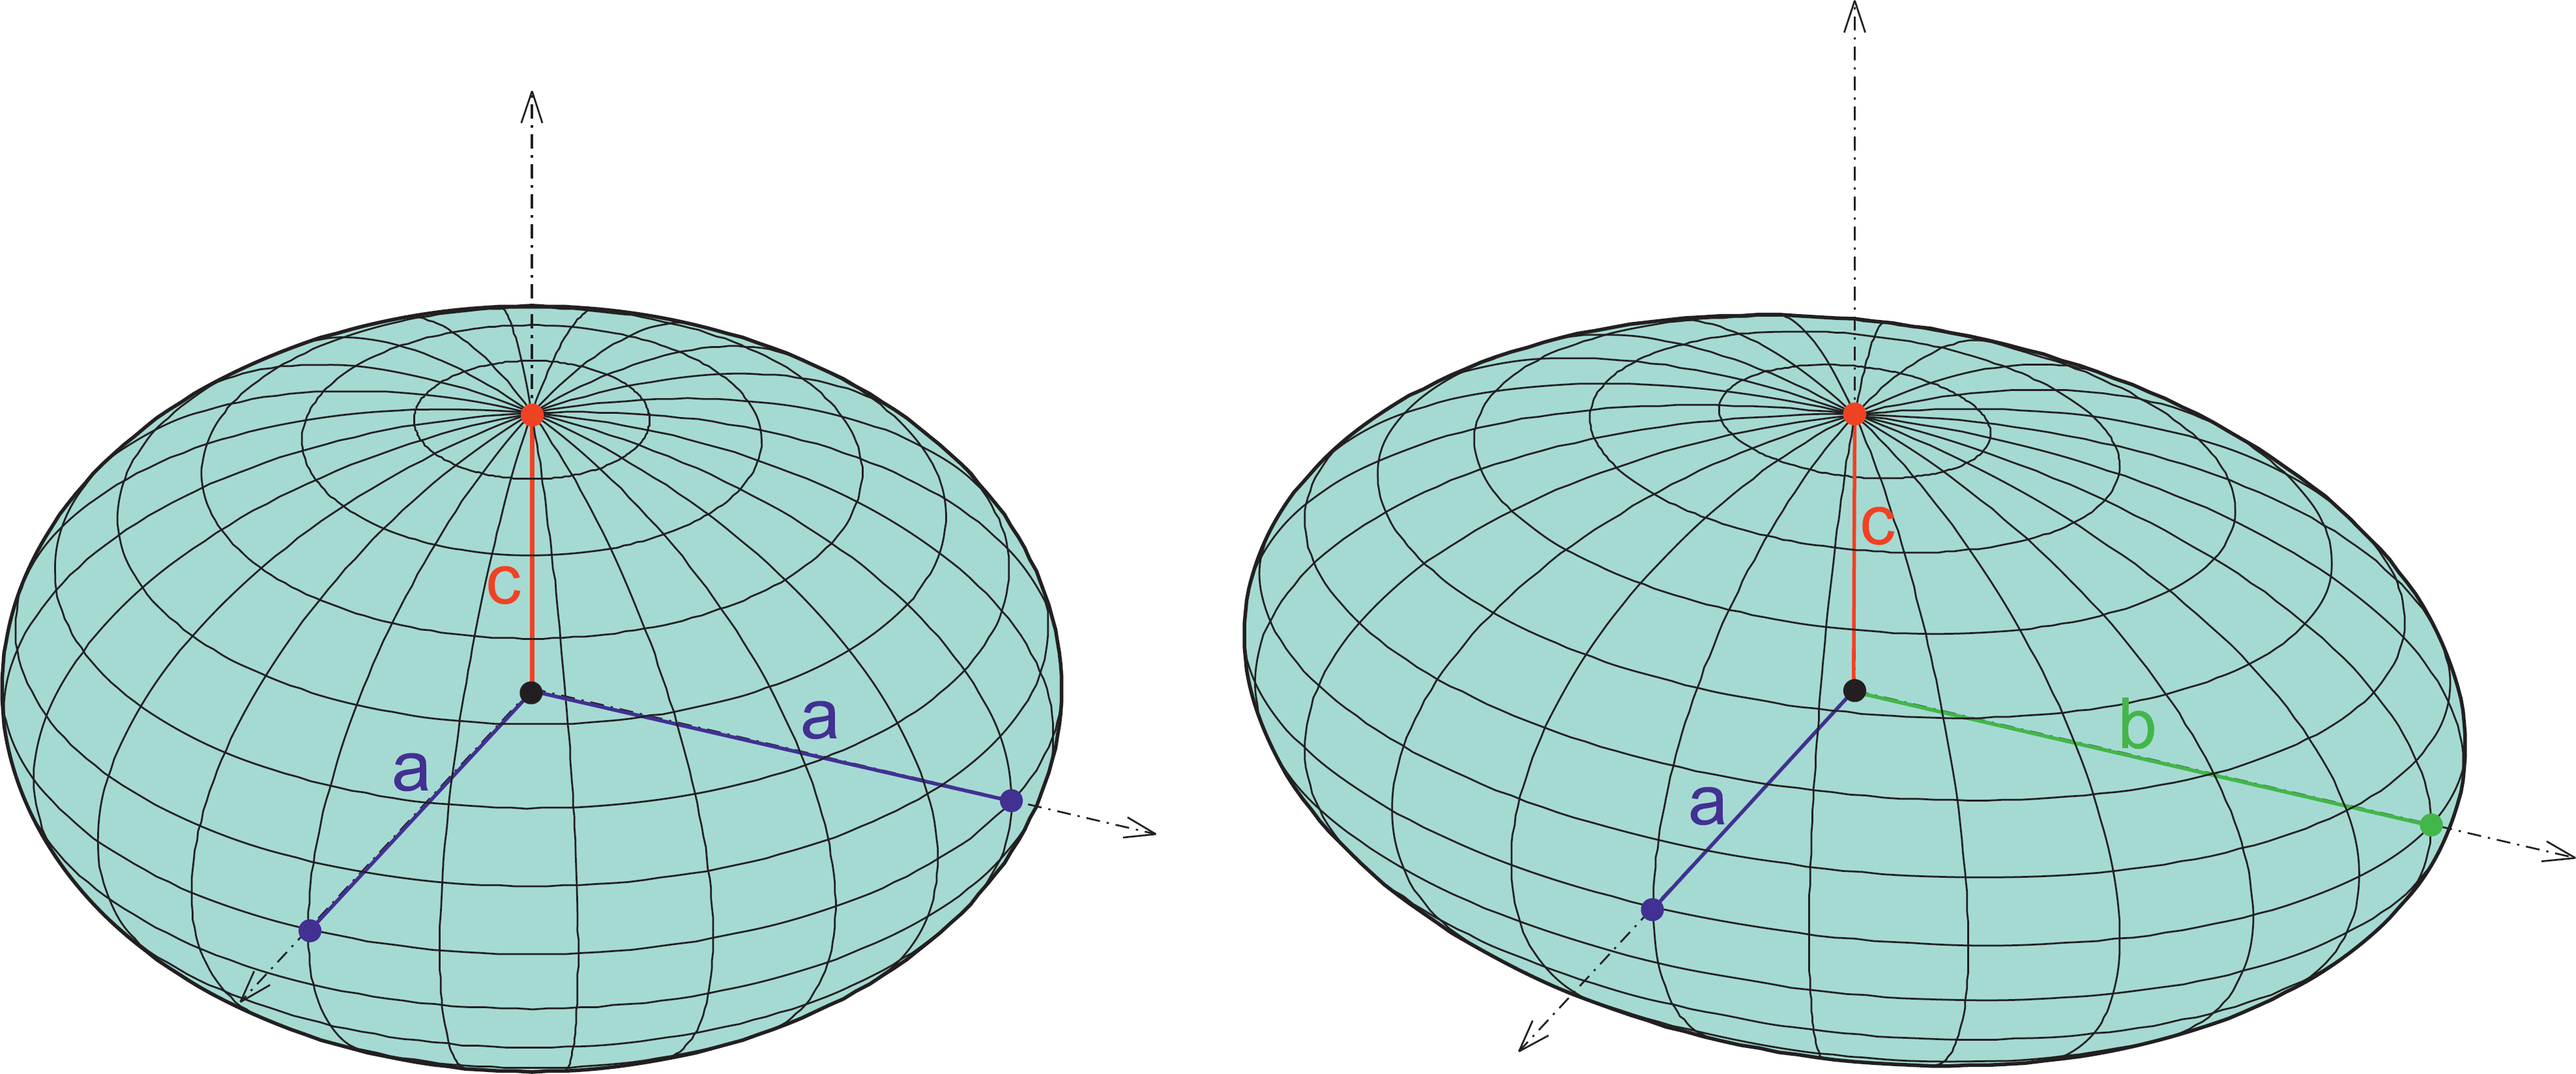
\includegraphics[width=0.85\textwidth]{../images/form_factor/Ellipsoid/Ellipsoide.png}
\end{center}
\caption{Ellipse of revolution (spheroid) and triaxial ellipse}
\label{fig:EllipsoidalObjects}
\end{figure}

The plugin "\texttt{ellipsoidal obj.}" contains form factors of ellipsoidal object with rotational symmetry, which are called ellipsoid of revolution or spheroid, as well as triaxial ellipsoidal objects. The three axes of the ellipsoids are assumed to be orthogonal. Because of the non-spherical symmetry of the objects an orientational average has to be performed for random oriented ellipsoids, which requires for spheroids a single integration and for triaxial ellipsoids a double integration. An optional integration over the size distribution would than slow down the numerical evaluation of the scattering intensity and care has to be taken, to use an appropriate integration routine. At the moment \SASfit makes use of the \texttt{pcubature} algorithm from Steven G. Johnson \cite{Johnson} instead of nested 1-dimensional integration routines used so far. Due to \SASfit internals an optional integration over the size distribution was realized via the form factor itself instead of including it via the GUI to profit from the speed-up of routines optimized for multi-dimensional integration.

\subsection{Ellipsoid of revolution or spheroid}
\label{sec:Spheroid}~\\

\begin{figure}[htb]
\begin{center}
%\includegraphics[width=0.706\textwidth,height=0.346\textwidth]{Elpsminr.png}
\includegraphics[width=0.5\textwidth,height=0.245\textwidth]{../images/form_factor/Ellipsoid/Elpsminr.png}
\end{center}
\caption{Ellipse, showing major and minor axes and parameters $a$ and $b$}
\label{minormajoraxes}
\end{figure}

An ellipsoid is a quadric surface in three dimensions obtained by
rotating an ellipse about one of its principal axes. Three
particular cases of an ellipsoid are:
\begin{itemize}
\item If the ellipse is rotated about its major axis, the surface is a prolate spheroid.
\item If the ellipse is rotated about its minor axis, the surface is an oblate spheroid.
\item If the generating ellipse is a circle, the surface is a sphere.
\end{itemize}

\begin{figure}[htb]
\begin{center}
\subfigure[oblate spheroid ($R_\mathrm{p} < R_\mathrm{e} $)]{\label{fig:oblateSpheroid}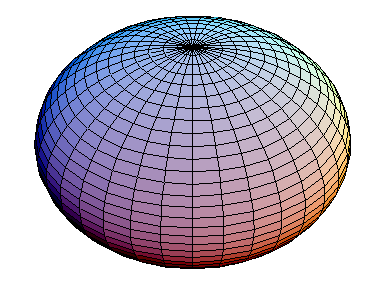
\includegraphics[width=0.48\textwidth]{../images/form_factor/Ellipsoid/OblateSpheroid.png}}
  \subfigure[prolate spheroid ($R_\mathrm{p} > R_\mathrm{e} $)]{\label{fig:prolateSpheroid}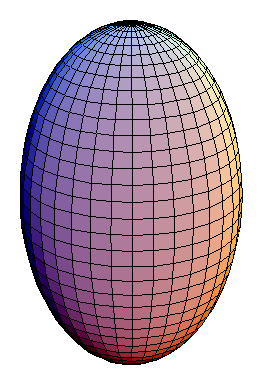
\includegraphics[width=0.48\textwidth]{../images/form_factor/Ellipsoid/ProlateSpheroid.png}}
\end{center}
\caption{A spheroid is an ellipsoid having two equal equatorial semi-axes $R_\mathrm{e}$. If the equatorial
semi-axis are larger than the principal axis $R_\mathrm{p}$ the spheroid becomes oblate (a), if they are smaller
it becomes prolate (b) and if they are equal the spheroid becomes a perfect sphere}
\label{prolate oblate}
\end{figure}

The orientational averaged scattering amplitude and scattering intensity are given by \cite{Guinier1939}
\begin{align}
\left\langle F_\text{spheroid}(Q,R_\mathrm{p},R_\mathrm{e},\Delta\eta)\right\rangle &= V\Delta\eta
 \int_0^{1}\! K\left(Q\sqrt{R_\mathrm{p}^2y^2+R_\mathrm{e}^2(1-y)^2}\right) \, \mathrm{d}y \\
I_\text{spheroid}(Q,R_\mathrm{p},R_\mathrm{e},\Delta\eta) &=  V^2\Delta\eta^2
 \int_0^{1}\! K^2\left(Q\sqrt{R_\mathrm{p}^2y^2+R_\mathrm{e}^2(1-y)^2}\right) \, \mathrm{d}y
\end{align}
with
\begin{align}
V &= \frac{4}{3}\pi R_\mathrm{e}^2R_\mathrm{p}\\
K(x) &= 3 \frac{\sin x - x \cos x}{x^3}\\
\Delta \eta &= \eta_\mathrm{core}-\eta_\mathrm{solv}
\end{align}
%$\lim_{Q=0} I_\text{spheroid}(Q,R_\mathrm{p},R_\mathrm{e},\Delta\eta)= \left( \frac{4}{3}\pi
%R_\mathrm{e}^2R_\mathrm{p} \Delta\eta \right)^2 $

The form factor of a spheroid has been implemented in three parametrisation variants.
The variants \texttt{spheroid V} and \texttt{spheroid nu} replace the old variants \texttt{Ellipsoid i} and \texttt{Ellipsoid ii}, which are not anymore available. \texttt{spheroid R} is a new parametrisation variant. Their input parameters are

~\\
\underline{Input Parameters for model \texttt{spheroid nu}:}
\begin{description}
\item[\texttt{nu}]
ratio between radius of the polar axes and equatorial axis.
Values of $\nu<1$ describe oblate ellipsoids, a value of $\nu=1$ a
sphere, and $\nu>1$ a prolate ellipsoids.
\item[\texttt{R\_equatorial}] length of the equatorial semi-axes $R_\mathrm{e}$
\item[\texttt{dummy}] not used
\item[\texttt{dummy}] not used
\item[\texttt{dummy}] not used
\item[\texttt{eta\_core}] scattering length density of spheroid
\item[\texttt{dummy}] not used
\item[\texttt{eta\_sol}] scattering length density of solvent
\end{description}
~\\
\underline{Input Parameters for model \texttt{spheroid V}:}
\begin{description}
\item[\texttt{V}] volume of spheroid
\item[\texttt{R\_equatorial}] length of equatorial semi-axes $R_\mathrm{e}$
\item[\texttt{dummy}] not used
\item[\texttt{dummy}] not used
\item[\texttt{dummy}] not used
\item[\texttt{eta\_core}] scattering length density of spheroid
\item[\texttt{dummy}] not used
\item[\texttt{eta\_sol}] scattering length density of solvent
\end{description}
~\\
\underline{Input Parameters for model \texttt{spheroid R}:}
\begin{description}
\item[\texttt{R\_polar}] length of polar semi-axis $R_\mathrm{p}$
\item[\texttt{R\_equatorial}] length of equatorial semi-axes $R_\mathrm{e}$
\item[\texttt{dummy}] not used
\item[\texttt{dummy}] not used
\item[\texttt{dummy}] not used
\item[\texttt{eta\_core}] scattering length density of spheroid
\item[\texttt{dummy}] not used
\item[\texttt{eta\_sol}] scattering length density of solvent
\end{description}


\begin{figure}[htb]
\begin{center}
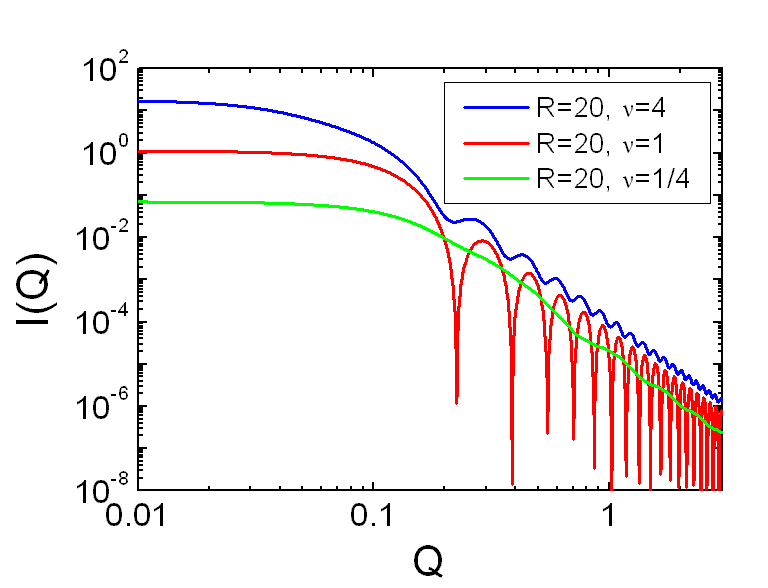
\includegraphics[width=0.768\textwidth,height=0.588\textwidth]{../images/form_factor/Ellipsoid/ellipsoid_ii.png}
\end{center}
\caption{form factor of an ellipsoid with axis $R$, $R$ and $\nu
R$.} \label{fig:I_ellipsoid_ii}
\end{figure}


%%%%%%%%%%%%%%%%%%%%%%%%%%%%%%%%%%%%%%%%%%%%%%%%%%%%%%%%
\clearpage
\subsection{Ellipsoid with two equal equatorial semi-axis $R$ and volume $V$}
\label{sect:Ellipsoid_i} ~\\

\begin{align}
I_\text{i}(Q,R,\nu) = \left( V \Delta\eta
\right)^2
 \int_0^{\frac{\pi}{2}}\! K^2\left(Q,R\sqrt{\nu^2\cos^2\Theta+\sin^2\Theta}\right)\sin\Theta\, d\Theta
\end{align}
with
$$
\nu=\frac{V}{R^3}\frac{3}{4\pi} \quad \mbox{so that}\quad V =\frac{4}{3}\pi\nu R^3
$$
and $\DS \lim_{Q=0} I_\text{i}(Q,R,\nu)= \left(V\Delta\eta\right)^2$

~\\
\underline{Input Parameters for model \texttt{Ellipsoid i}:}
\begin{description}
\item[\texttt{R}] radius of the rotational axes
\item[\texttt{V}] total volume of the ellipsoid.
\end{description}

\begin{figure}[htb]
\begin{center}
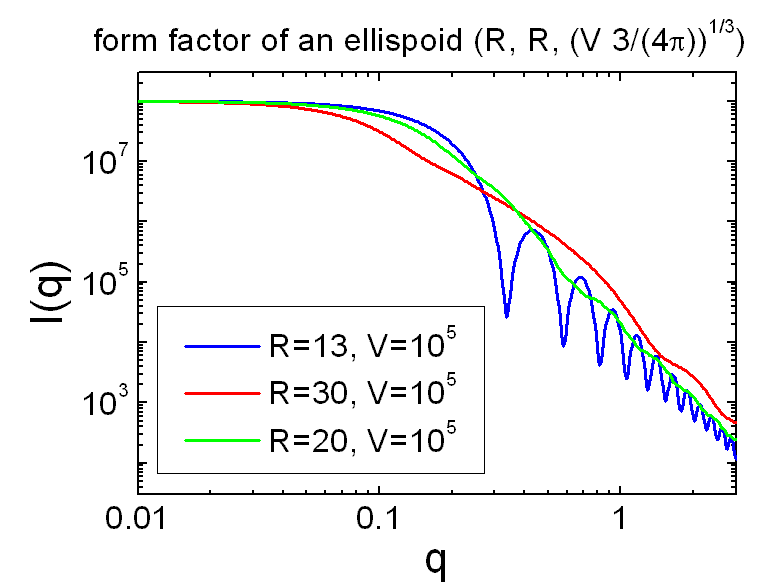
\includegraphics[width=0.768\textwidth,height=0.588\textwidth]{../images/form_factor/Ellipsoid/ellipsoid_i.png}
\end{center}
\caption{form factor of an ellipsoid with axis $R$, $R$ and
$\oldsqrt[3]{V\frac{3}{4\pi}}$.} \label{fig:I_ellipsoid_i}
\end{figure}

%%%%%%%%%%%%%%%%%%%%%%%%%%%%%%%%%%%%%%%%%%%%%%%%%%%%%%%%
\clearpage
\subsection{Ellipsoidal core shell structure}
\label{sect:EllipsoidalCoreShell} ~\\
For these form factor plugins a size distribution parameter has been included directly in the form factor to avoid applying nested numerical integration routines. A routine for multi-dimensional integration (\texttt{pcubature} \cite{Johnson}) has been used instead.
\begin{figure}[htb]
\begin{center}
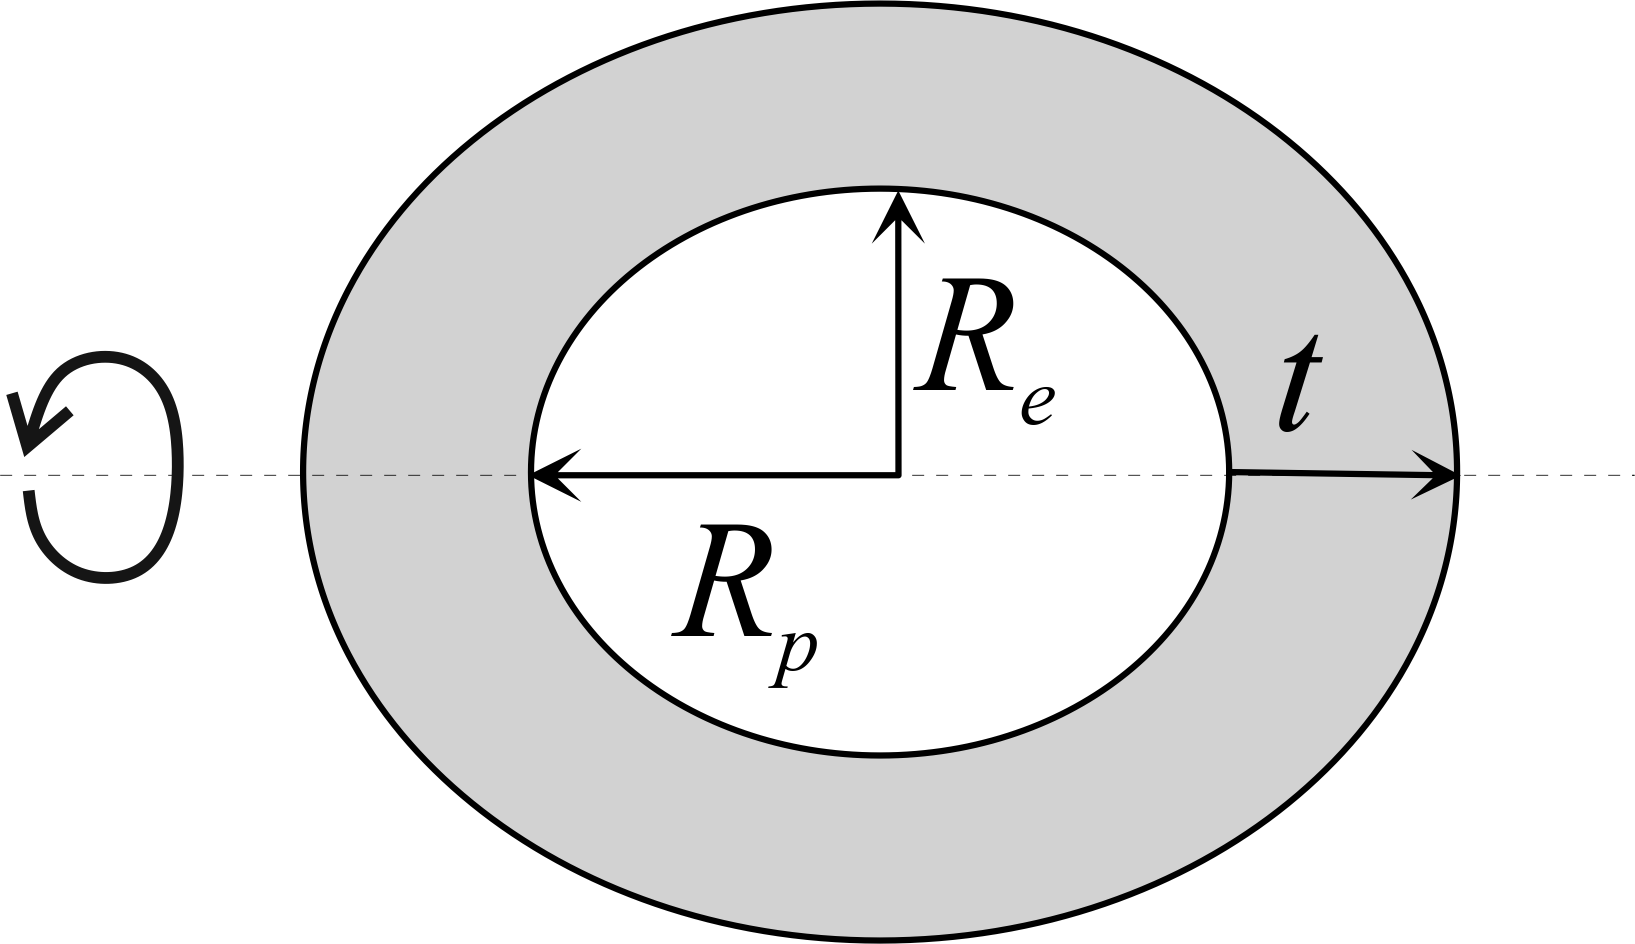
\includegraphics[width=0.5\textwidth,height=0.28855\textwidth]{../images/form_factor/Ellipsoid/ellipsoidalShell.png}
\end{center}
\caption{Ellipsoid of revolution with an outer shell of constant thickness $t$} \label{ellipsoidalShell}
\end{figure}
\begin{align}
I_\text{ECSh}(Q,R_\mathrm{p},R_\mathrm{e},t) = \left\langle F^2(Q,R_\mathrm{p},R_\mathrm{e},t) \right\rangle
& = \int_0^1 \left[F(Q,R_\mathrm{p},R_\mathrm{e},t,\mu)\right]^2 d\mu \\
\left\langle F(Q,R_\mathrm{p},R_\mathrm{e},t) \right\rangle & = \int_0^1 F(Q,R_\mathrm{p},R_\mathrm{e},t,\mu)
d\mu
\end{align}
with
\begin{align}
F(Q,R_\mathrm{p},R_\mathrm{e},t,\mu) &= \left(\eta_\text{core}-\eta_\text{shell}\right) V_c\left[
\frac{3j_1(x_c)}{x_c}\right]
          +\left(\eta_\text{shell}-\eta_\text{sol}\right) V_t\left[ \frac{3j_1(x_t)}{x_t}\right]
          \nonumber \\
j_1(x) &= \frac{\sin(x)-x\cos(x)}{x^2} \nonumber \\
x_c &= Q \sqrt{R_\mathrm{p}^2\mu^2+R_\mathrm{e}^2(1-\mu^2)} \nonumber \\
x_t &= Q \sqrt{(R_\mathrm{p}+t)^2\mu^2+(R_\mathrm{e}+t)^2(1-\mu^2)} \nonumber \\
V_c &= \frac{4}{3}\pi R_\mathrm{p}R_\mathrm{e}^2 \nonumber \\
V_t &= \frac{4}{3}\pi (R_\mathrm{p}+t)(R_\mathrm{e}+t)^2 \nonumber
\end{align}
\begin{align}
\eta_\text{core} &: \text{scattering length density of core} \nonumber \\
\eta_\text{shell} &: \text{scattering length density of shell} \nonumber \\
\eta_\text{sol} &: \text{scattering length density of solvent} \nonumber \\
R_\mathrm{p} &: \text{polar semi-axes of elliptical core} \nonumber \\
R_\mathrm{e} &: \text{equatorial semi-axis of elliptical core} \nonumber \\
t &: \text{thickness of shell} \nonumber \\
V_c &: \text{volume of core} \nonumber \\
V_t &: \text{total volume of core along with shell} \nonumber
\end{align}

Several variants including a size distribution have been implemented which just differ if only none, one or both axis scale with the same size distribution and if additionally also scales with that distribution.
\begin{align*}
\text{\texttt{Ellipsoidal Shell}}           &:                                            \left\langle F^n(Q,R_\mathrm{p},R_\mathrm{e},t)\right\rangle\\
\text{\texttt{Ellipsoidal Shell (t)}}       &: \int_0^\infty \mathrm{LogNorm}(\nu,\sigma) \left\langle F^n(Q,R_\mathrm{p},R_\mathrm{e},\nu t)\right\rangle \mathrm{d}\nu\\
\text{\texttt{Ellipsoidal Shell (Rp)}}      &: \int_0^\infty \mathrm{LogNorm}(\nu,\sigma) \left\langle F^n(Q,\nu R_\mathrm{p},R_\mathrm{e}, t)\right\rangle \mathrm{d}\nu\\
\text{\texttt{Ellipsoidal Shell (Rp t)}}    &: \int_0^\infty \mathrm{LogNorm}(\nu,\sigma) \left\langle F^n(Q,\nu R_\mathrm{p},R_\mathrm{e},\nu t)\right\rangle \mathrm{d}\nu\\
\text{\texttt{Ellipsoidal Shell (Re)}}      &: \int_0^\infty \mathrm{LogNorm}(\nu,\sigma) \left\langle F^n(Q,R_\mathrm{p},\nu R_\mathrm{e},t)\right\rangle \mathrm{d}\nu\\
\text{\texttt{Ellipsoidal Shell (Re t)}}    &: \int_0^\infty \mathrm{LogNorm}(\nu,\sigma) \left\langle F^n(Q,R_\mathrm{p},\nu R_\mathrm{e},\nu t)\right\rangle \mathrm{d}\nu\\
\text{\texttt{Ellipsoidal Shell (Re Rp)}}   &: \int_0^\infty \mathrm{LogNorm}(\nu,\sigma) \left\langle F^n(Q,\nu R_\mathrm{p},\nu R_\mathrm{e},t)\right\rangle \mathrm{d}\nu\\
\text{\texttt{Ellipsoidal Shell (Re Rp t)}} &: \int_0^\infty \mathrm{LogNorm}(\nu,\sigma) \left\langle F^n(Q,\nu R_\mathrm{p},\nu R_\mathrm{e},\nu t)\right\rangle \mathrm{d}\nu
\end{align*}
with $n$ being either 1 or 2 depending if the size averaged amplitude or the size averaged intensity needs to be calculated. As a size distribution a lognormal distribution is assumed where all parameters are scaled simultaneously. The used lognormal distribution is defined as
$$
\mathrm{LogNorm}(x,\sigma) = \frac{1}{\sqrt{2\pi}x} \exp\left(-\frac{\ln^2(x)}{2\sigma^2}\right)
$$
\vspace{0.5cm}
~\\
\underline{Input Parameters for model \texttt{Ellipsoidal Shell}:}
\begin{description}
\item[\texttt{R\_p}] semi-principal polar axes of elliptical core $R_\mathrm{p}$
\item[\texttt{R\_e}] equatorial semi-axis axes of elliptical core $R_\mathrm{e}$
\item[\texttt{dummy}] not used
\item[\texttt{t}] thickness of shell $t$
\item[\texttt{dummy}] not used
\item[\texttt{eta\_core}] scattering length density of core $\eta_\text{c}$
\item[\texttt{eta\_shell}] scattering length density of shell $\eta_\text{sh}$
\item[\texttt{eta\_sol}] scattering length density of solvent $\eta_\text{sol}$
\end{description}
~\\
\underline{Input Parameters for model \texttt{Ellipsoidal Shell (t)}, \texttt{Ellipsoidal Shell (Rp)},}
\underline{\texttt{Ellipsoidal Shell (Rp t)}, \texttt{Ellipsoidal Shell (Re)}, \texttt{Ellipsoidal Shell (Re t)},}
\underline{\texttt{Ellipsoidal Shell (Re Rp)}, \texttt{Ellipsoidal Shell (Re Rp t)}:}
\begin{description}
\item[\texttt{R\_p}] semi-principal polar axes of elliptical core $R_\mathrm{p}$
\item[\texttt{R\_e}] equatorial semi-axis axes of elliptical core $R_\mathrm{e}$
\item[\texttt{dummy}] not used
\item[\texttt{t}] thickness of shell $t$
\item[\texttt{sigma}] width of the LogNorm size distribution
\item[\texttt{eta\_core}] scattering length density of core $\eta_\text{c}$
\item[\texttt{eta\_shell}] scattering length density of shell $\eta_\text{sh}$
\item[\texttt{eta\_sol}] scattering length density of solvent $\eta_\text{sol}$
\end{description}

\begin{figure}[htb]
\begin{center}
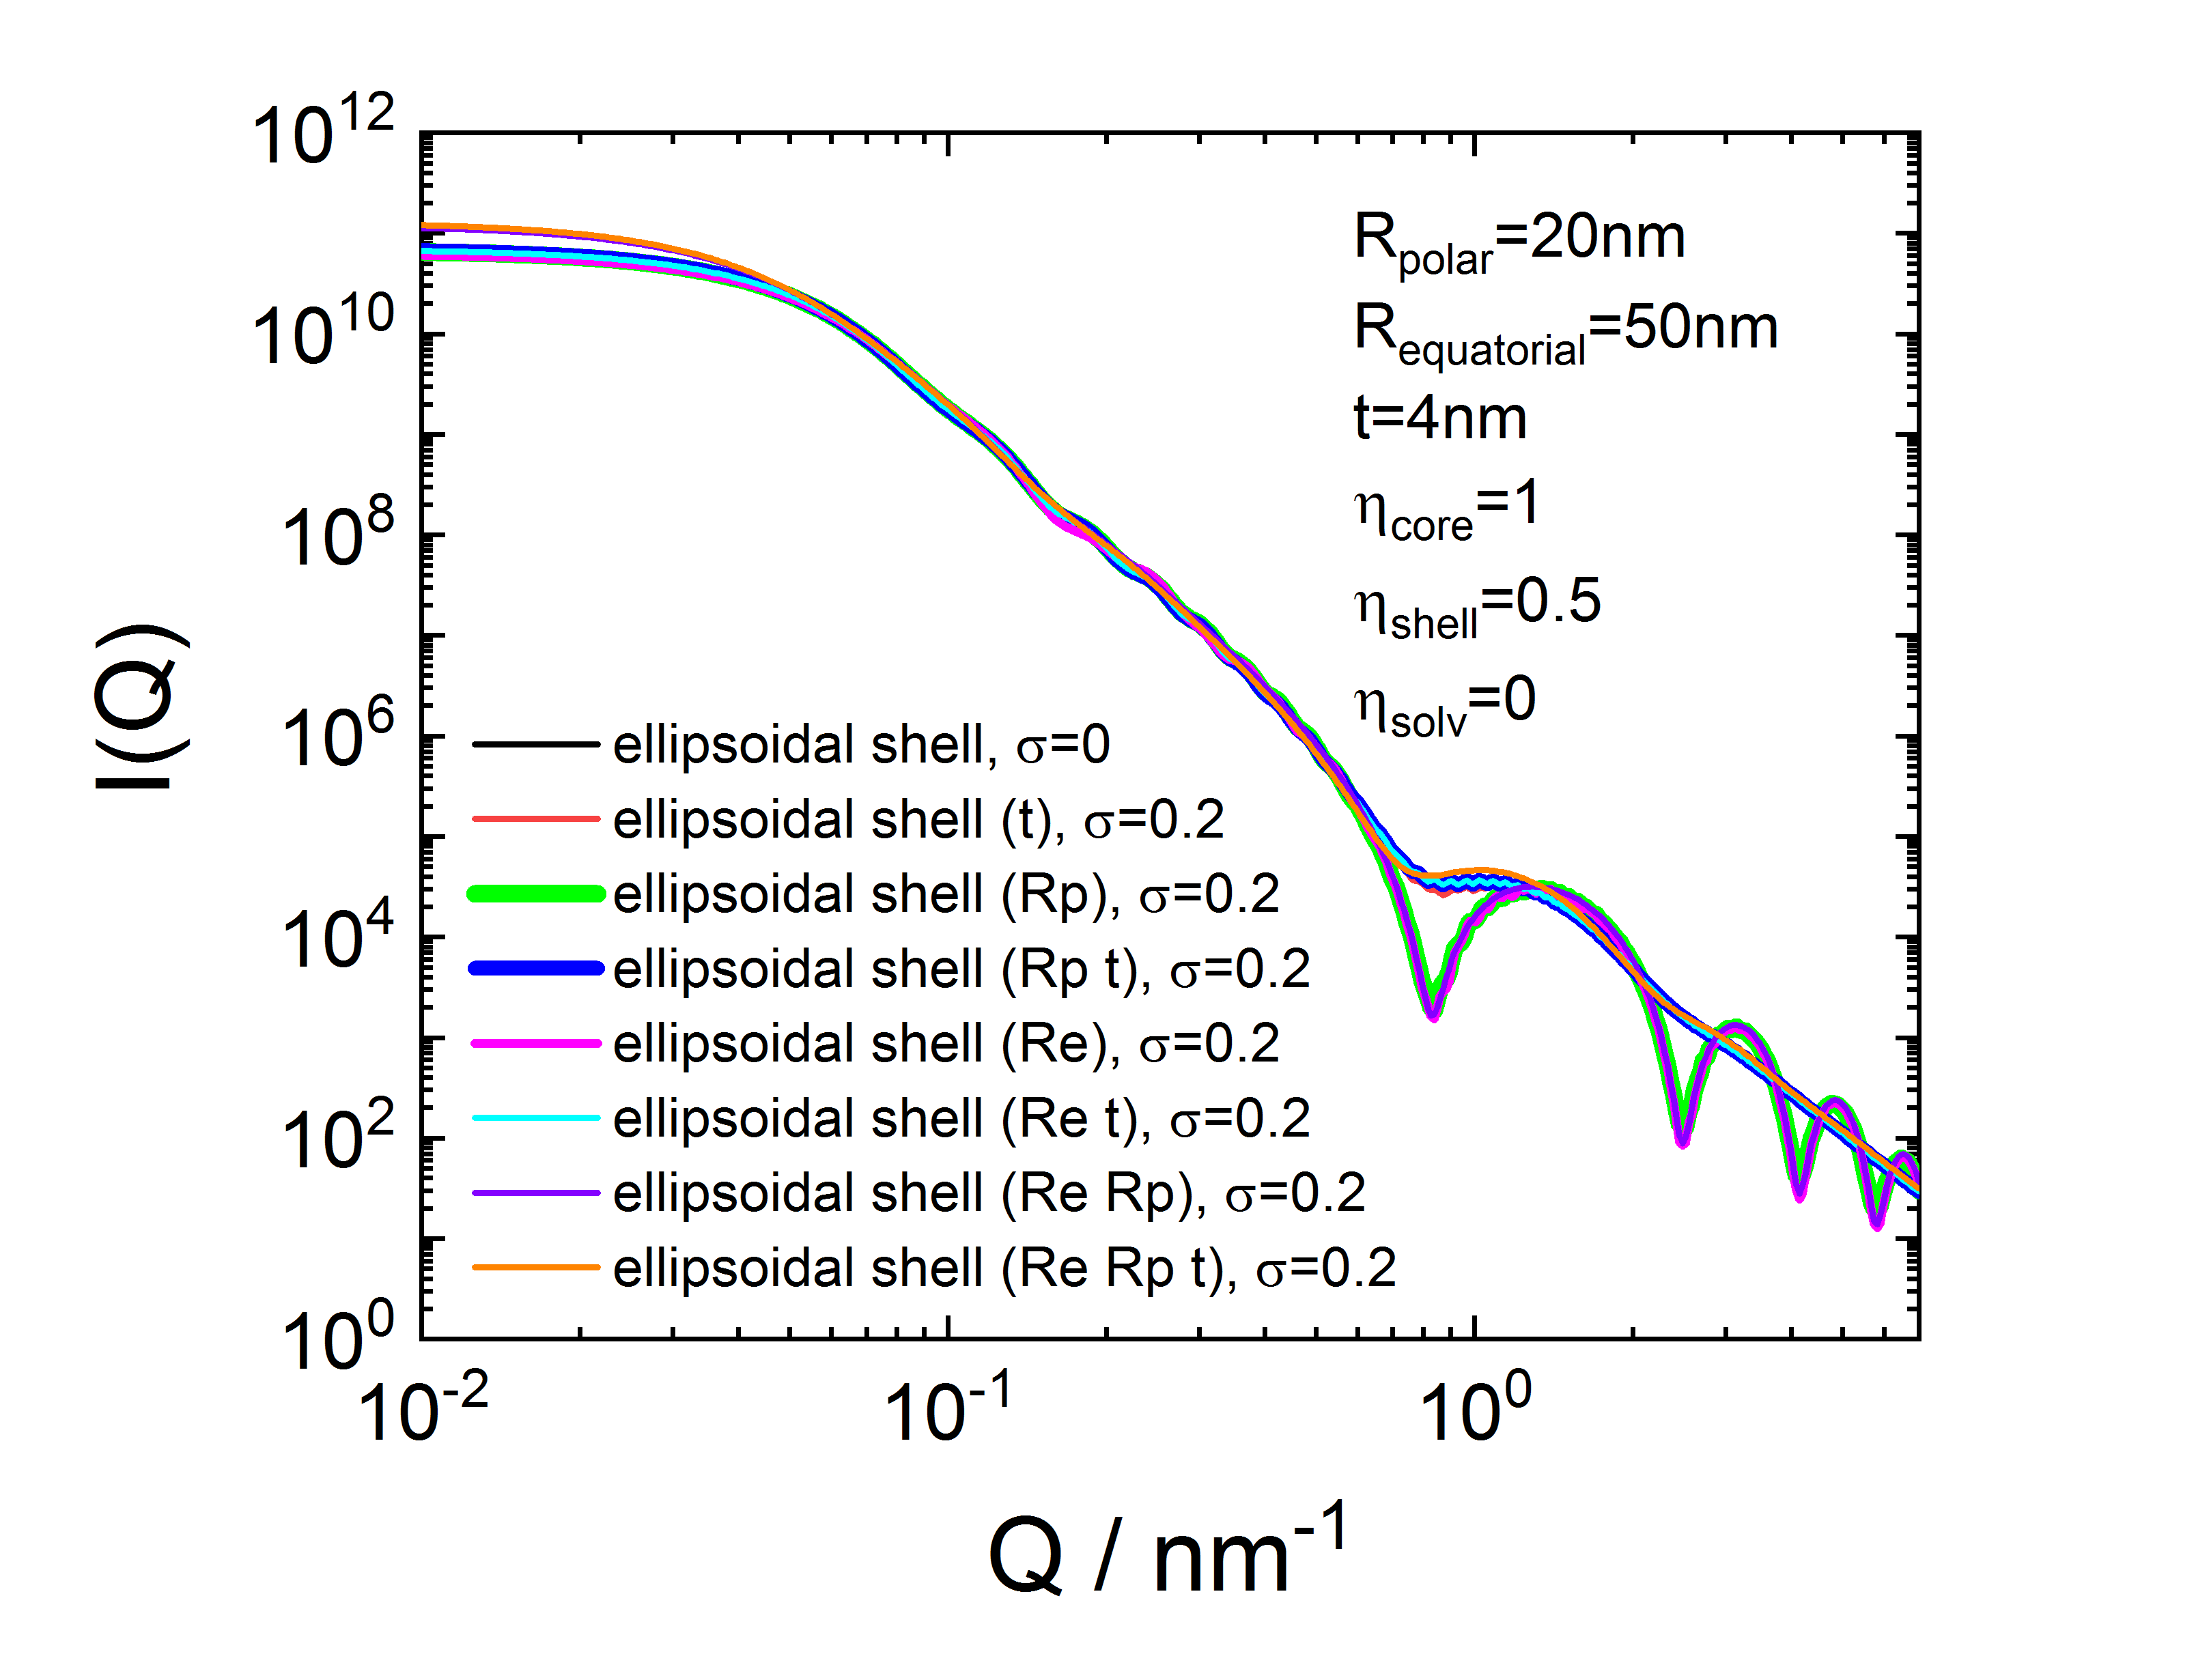
\includegraphics[width=0.768\textwidth,height=0.588\textwidth]{../images/form_factor/Ellipsoid/spheroid_core_shell.png}
\end{center}
\caption{Form factor of an ellipsoidal core shell structure including a lognormal size distribution.} \label{fig:I_ellipsoidal_core_shell}
\end{figure}


%%%%%%%%%%%%%%%%%%%%%%%%%%%%%%%%%%%%%%%%%%%%%%%%%%%%%%%%
\clearpage
\subsection{triaxial ellipsoidal core shell structure}
\label{sect:triaxEllShell1} ~\\
Also for these form factor plugins a size distribution parameter has been included directly in the form factor similar to the ellipsoidal shell of revolution to avoid applying nested numerical integration routines. As for the triaxial ellipsoid already a double integration for the orientational averaging is required it becomes even more important to have an optimized integration routine for including an additional size distribution, i.e an additional integration. The routine for multi-dimensional integration  (\texttt{pcubature} \cite{Johnson}) has been used.

\begin{figure}[htb]
\begin{center}
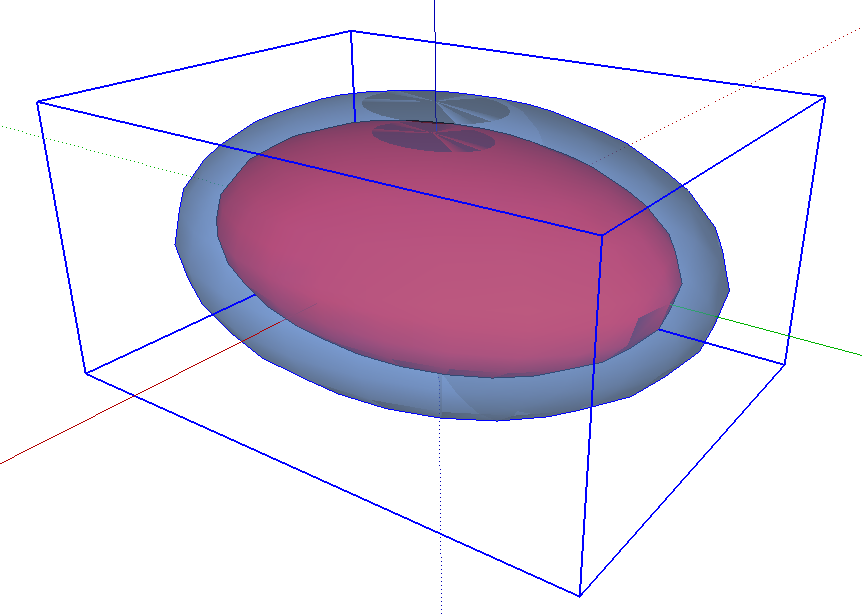
\includegraphics[width=0.45\textwidth,height=0.32177\textwidth]{../images/form_factor/Ellipsoid/triaxEll.png}
\hspace{0.08\textwidth}
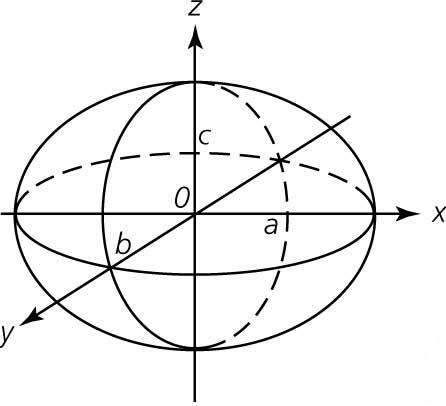
\includegraphics[width=0.45\textwidth,height=0.4096\textwidth]{../images/form_factor/Ellipsoid/A4ellipd.png}
\end{center}
\caption{triaxial ellipsoidal core shell structure} \label{triaEllShell}
\end{figure}

\begin{align}
I_\text{triaxEllSh}(Q) = \left\langle F^2(Q,a,b,c,t) \right\rangle &= \int^1_0 \int ^1_0 dx\,dy\, K_\text{sh}^2(Q,R,R_t)\\
\left\langle F(Q,a,b,c,t) \right\rangle & = \int^1_0 \int ^1_0 dx\,dy\, K_\text{sh}(Q,R,R_t)
\end{align}
with
\begin{align}
K(QR)         &= 3 \frac{\sin QR - QR\cos QR}{(QR)^3} \\
K_\text{sh}(Q,R,R_t) &= \left(\eta_\text{c}-\eta_\text{sh}\right)K(QR)+\left(\eta_\text{sh}-\eta_\text{sol}\right)K(QR_t) \\
R^2 &= \left[a^2\cos^2\left(\pi x/2\right) + b^2\sin^2\left(\pi x/2\right)\right](1-y^2)+c^2y^2 \nonumber \\
R_t^2 &= \left[(a+t)^2\cos^2\left(\pi x/2\right) + (b+t)^2\sin^2\left(\pi x/2\right)\right](1-y^2)+(c+t)^2y^2
\nonumber \\
V_c &= \frac{4}{3}\pi abc \nonumber \\
V_t &= \frac{4}{3}\pi (a+t)(b+t)(c+t) \nonumber
\end{align}
\begin{align}
\eta_\text{c} &: \text{scattering length density of core} \nonumber \\
\eta_\text{sh} &: \text{scattering length density of shell} \nonumber \\
\eta_\text{sol} &: \text{scattering length density of solvent} \nonumber \\
a &: \text{semi-axes of elliptical core} \nonumber \\
b &: \text{semi-axes of elliptical core} \nonumber \\
c &: \text{semi-axes of elliptical core} \nonumber \\
t &: \text{thickness of shell} \nonumber \\
V_c &: \text{volume of core} \nonumber \\
V_t &: \text{total volume of core along with shell} \nonumber
\end{align}

Several variants including a size distribution have been implemented which just differ if only none, one or both axis scale with the same size distribution and if additionally also scales with that distribution.
\begin{align*}
\text{\texttt{triax ellip shell}}     &:                                            \left\langle F^n(Q,    a,    b,    c,    t)\right\rangle\\
\text{\texttt{triax ellip shell t}}   &: \int_0^\infty \mathrm{LogNorm}(\nu,\sigma) \left\langle F^n(Q,    a,    b,    c,\nu t)\right\rangle \mathrm{d}\nu\\
\text{\texttt{triax ellip shell 1}}   &: \int_0^\infty \mathrm{LogNorm}(\nu,\sigma) \left\langle F^n(Q,\nu a,    b,    c,    t)\right\rangle \mathrm{d}\nu\\
\text{\texttt{triax ellip shell 1t}}  &: \int_0^\infty \mathrm{LogNorm}(\nu,\sigma) \left\langle F^n(Q,\nu a,    b,    c,\nu t)\right\rangle \mathrm{d}\nu\\
\text{\texttt{triax ellip shell 2}}   &: \int_0^\infty \mathrm{LogNorm}(\nu,\sigma) \left\langle F^n(Q,\nu a,\nu b,    c,    t)\right\rangle \mathrm{d}\nu\\
\text{\texttt{triax ellip shell 2t}}  &: \int_0^\infty \mathrm{LogNorm}(\nu,\sigma) \left\langle F^n(Q,\nu a,\nu b,    c,\nu t)\right\rangle \mathrm{d}\nu\\
\text{\texttt{triax ellip shell 3}}   &: \int_0^\infty \mathrm{LogNorm}(\nu,\sigma) \left\langle F^n(Q,\nu a,\nu b,\nu c,    t)\right\rangle \mathrm{d}\nu\\
\text{\texttt{triax ellip shell 3t}}  &: \int_0^\infty \mathrm{LogNorm}(\nu,\sigma) \left\langle F^n(Q,\nu a,\nu b,\nu c,\nu t)\right\rangle \mathrm{d}\nu
\end{align*}
with $n$ being either 1 or 2 depending if the size averaged amplitude or the size averaged intensity needs to be calculated. As a size distribution a lognormal distribution is assumed where all parameters are scaled simultaneously. The used lognormal distribution is defined as
$$
\mathrm{LogNorm}(x,\sigma) = \frac{1}{\sqrt{2\pi}x} \exp\left(-\frac{\ln^2(x)}{2\sigma^2}\right)
$$

\vspace{3cm}
\noindent \underline{Input Parameters for model \texttt{triax ellip shell}:}
\begin{description}
\item[\texttt{a}] semi-axes of elliptical core $a$
\item[\texttt{b}] semi-axes of elliptical core $b$
\item[\texttt{c}] semi-axes of elliptical core $c$
\item[\texttt{t}] thickness of shell $t$
\item[\texttt{dummy}] not used
\item[\texttt{eta\_c}] scattering length density of core $\eta_\text{c}$
\item[\texttt{eta\_sh}] scattering length density of shell $\eta_\text{sh}$
\item[\texttt{eta\_sol}] scattering length density of solvent $\eta_\text{sol}$
\end{description}
~\\
\underline{Input Parameters for model \texttt{triax ellip shell t}, \texttt{triax ellip shell 1},}
\underline{\texttt{triax ellip shell 1t}, \texttt{triax ellip shell 2}, \texttt{triax ellip shell 2t},}
\underline{\texttt{triax ellip shell 3}, \texttt{triax ellip shell 3t}}:
\begin{description}
\item[\texttt{a}] semi-axes of elliptical core $a$
\item[\texttt{b}] semi-axes of elliptical core $b$
\item[\texttt{c}] semi-axes of elliptical core $c$
\item[\texttt{t}] thickness of shell $t$
\item[\texttt{sigma}] width of the LogNorm size distribution $\sigma$
\item[\texttt{eta\_c}] scattering length density of core $\eta_\text{c}$
\item[\texttt{eta\_sh}] scattering length density of shell $\eta_\text{sh}$
\item[\texttt{eta\_sol}] scattering length density of solvent $\eta_\text{sol}$
\end{description}

\begin{figure}[htb]
\begin{center}
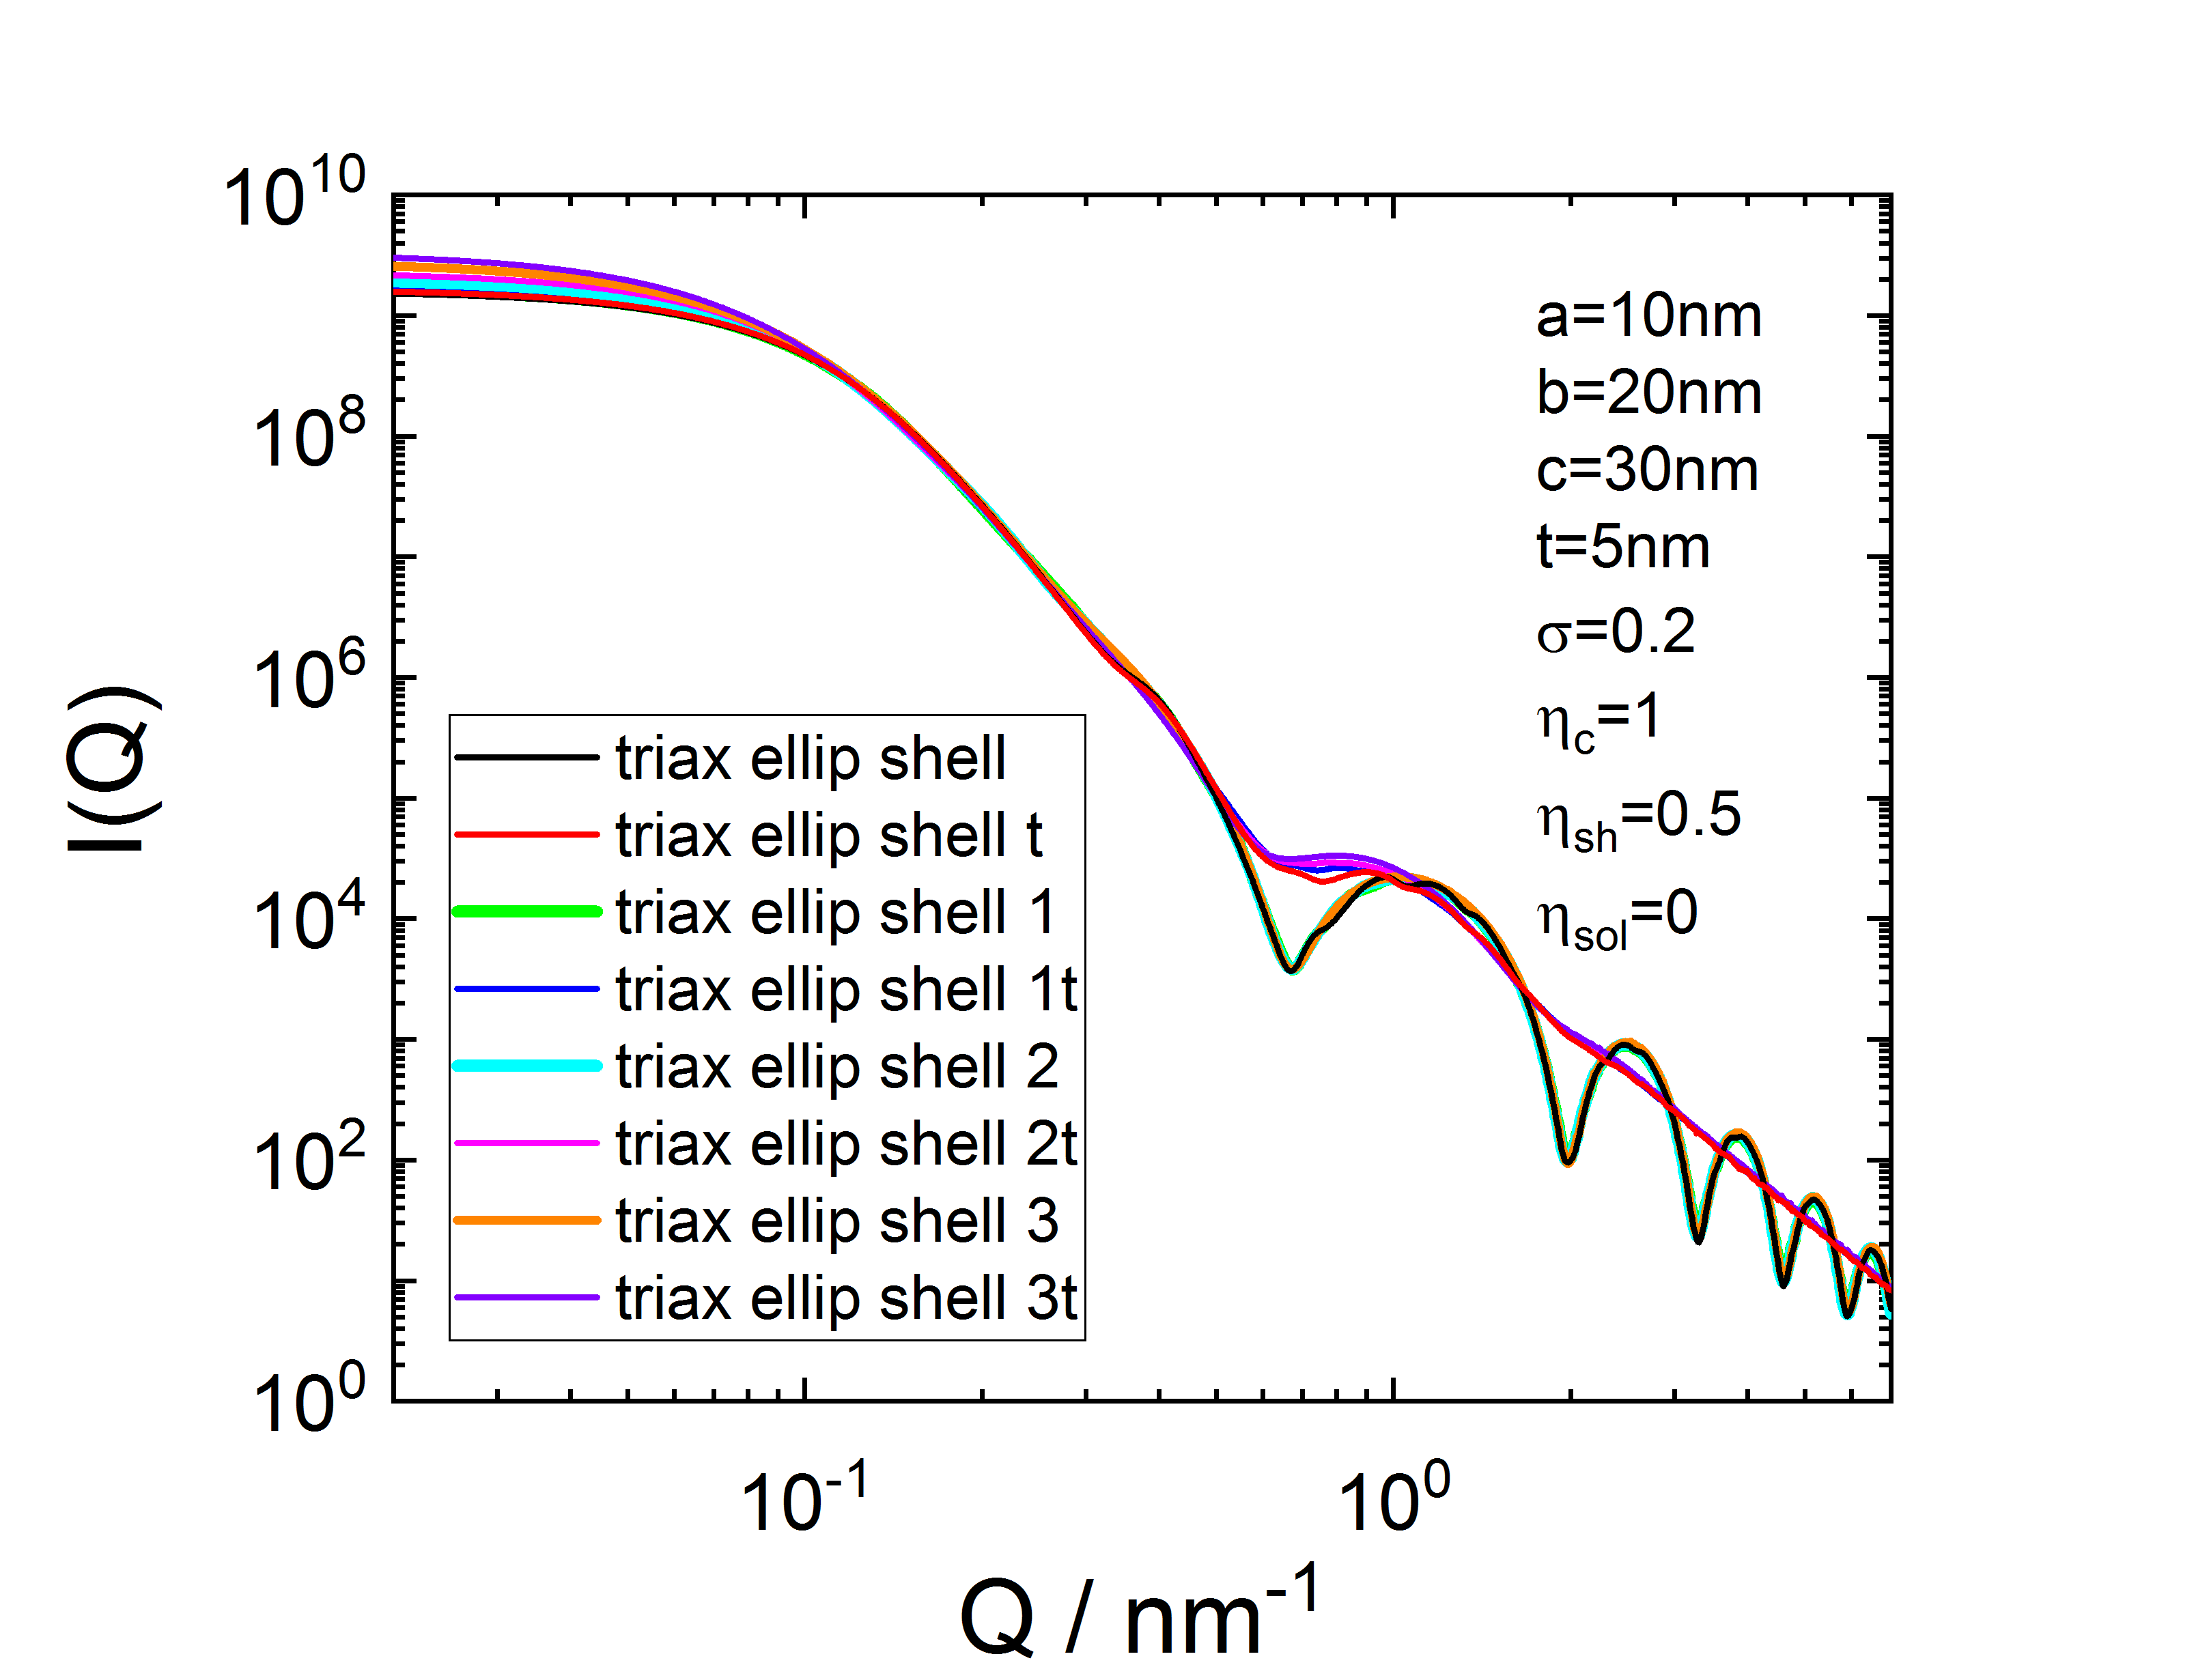
\includegraphics[width=0.48\textwidth]{../images/form_factor/Ellipsoid/triax_ellipsoidal_core_shell_1.png}
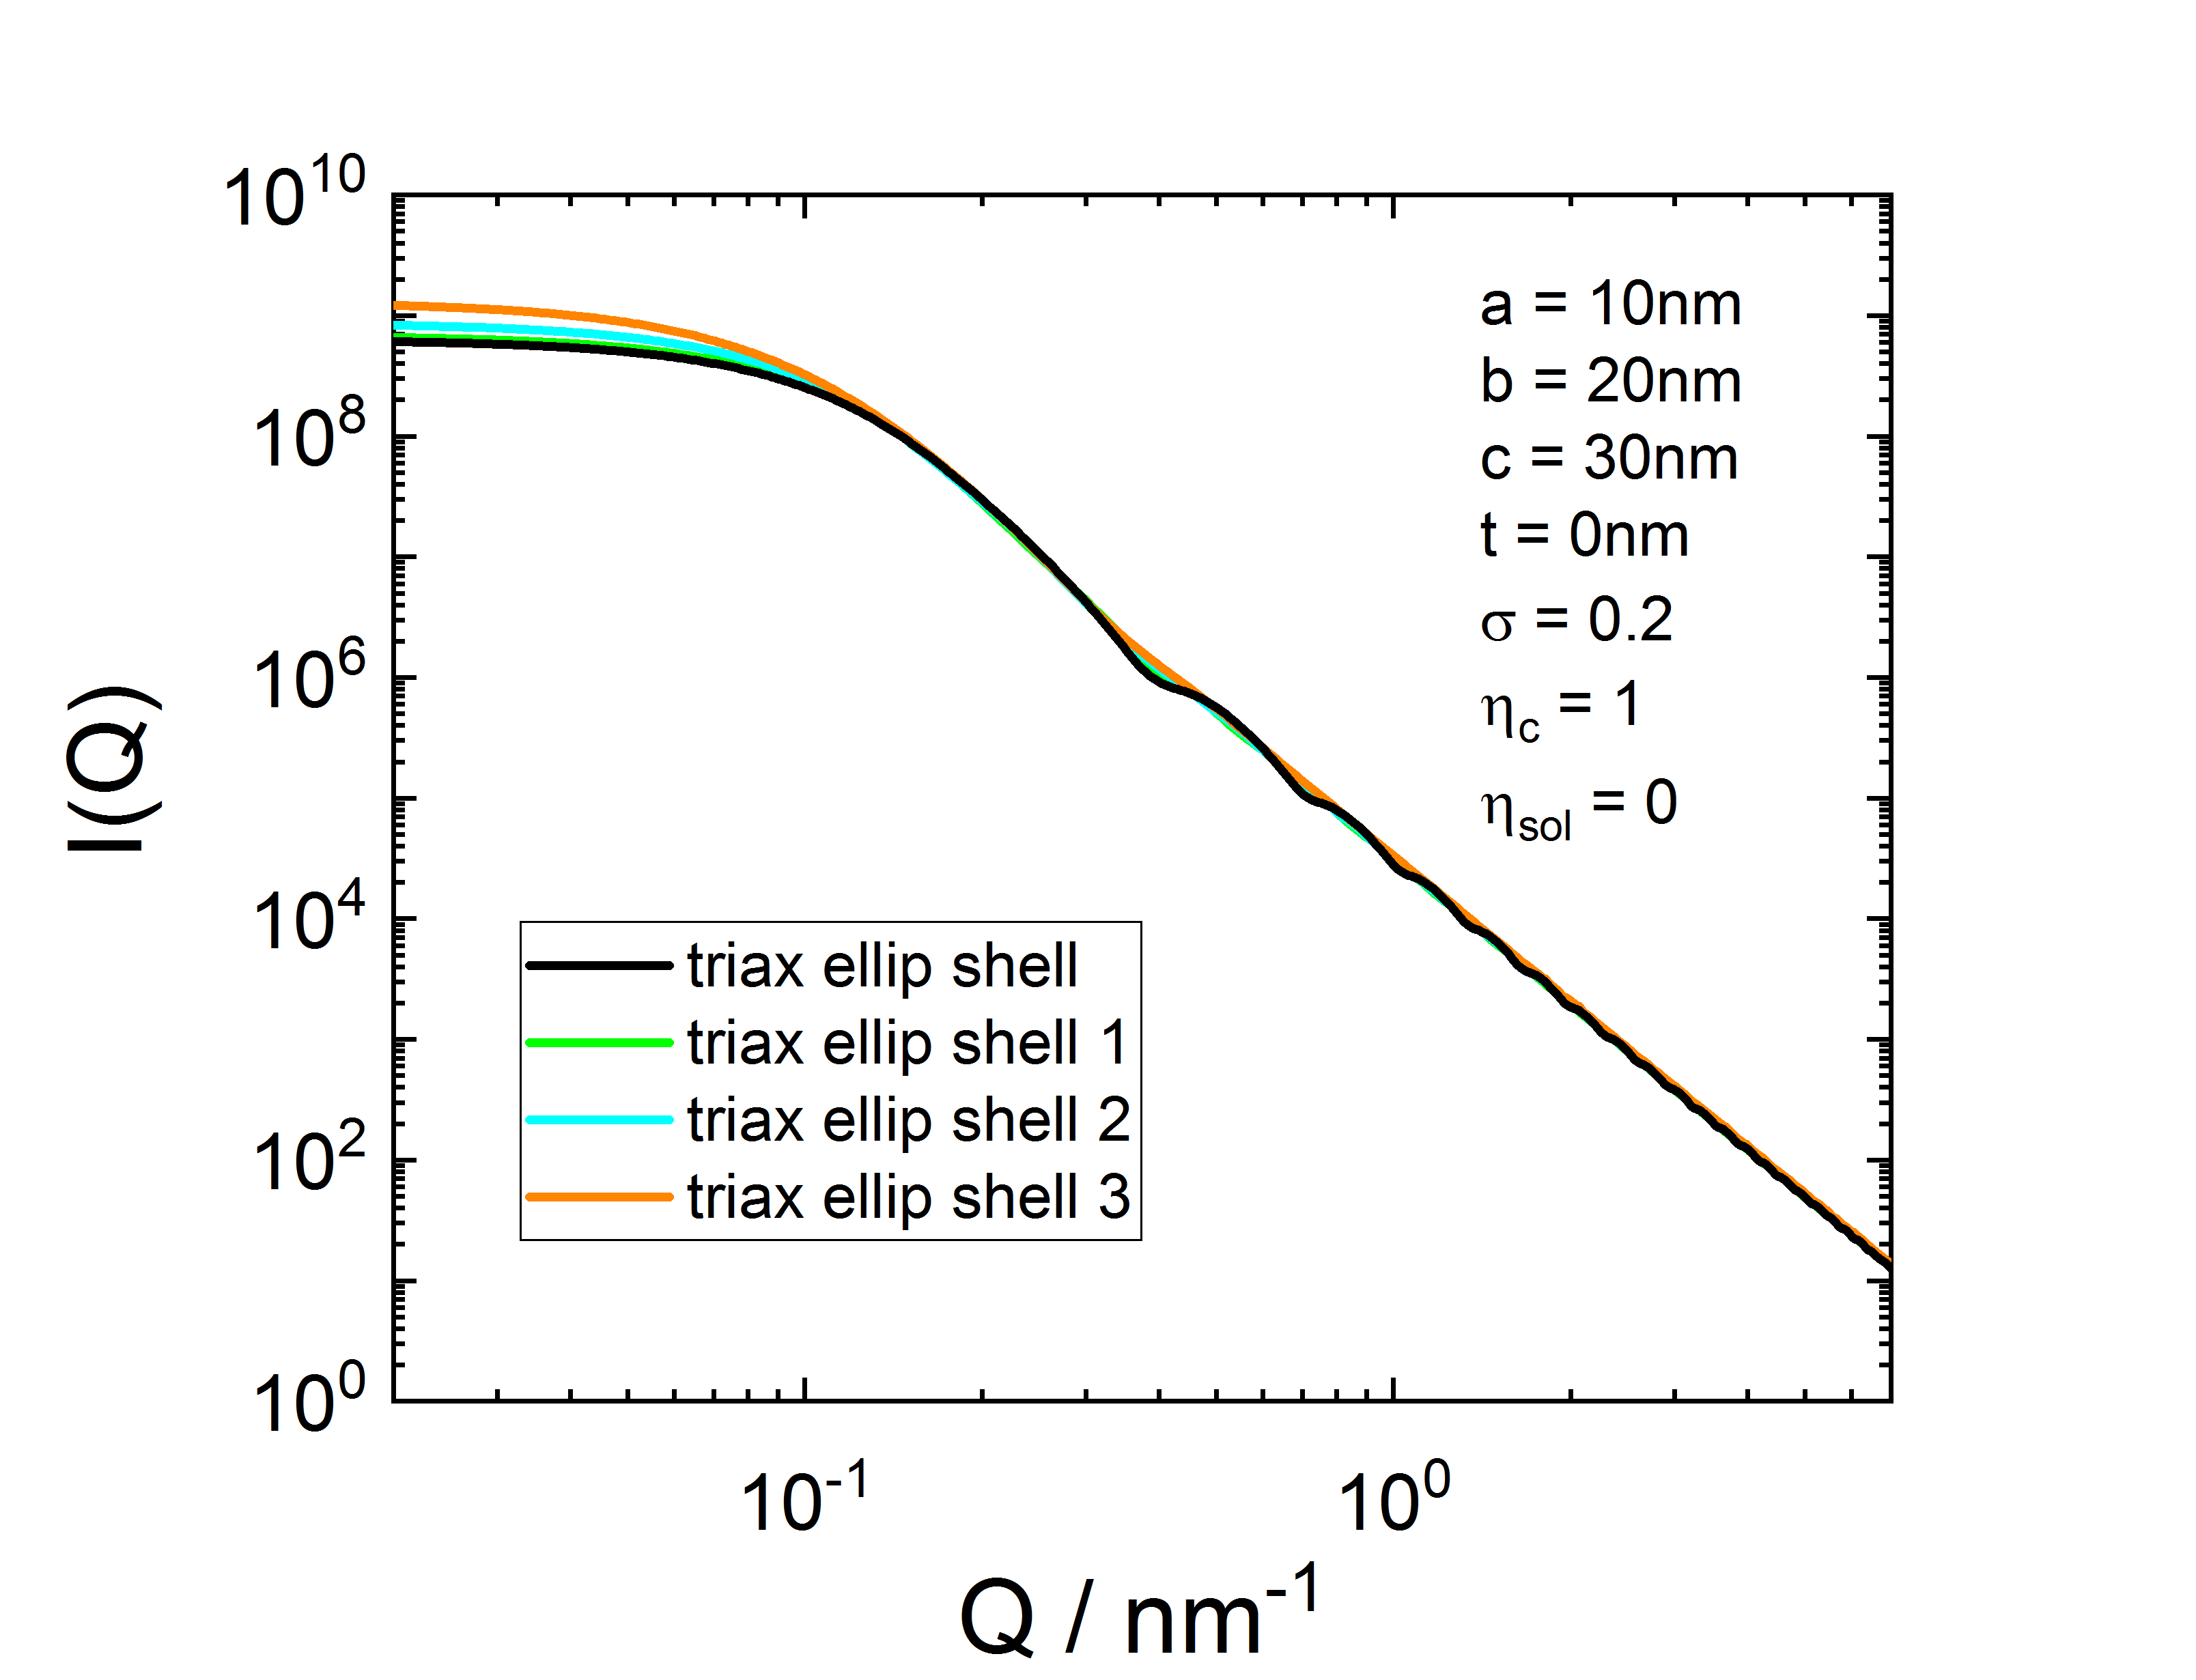
\includegraphics[width=0.48\textwidth]{../images/form_factor/Ellipsoid/triax_ellipsoidal_core_shell_2.png}
\end{center}
\caption{Form factor of a triaxial ellipsoidal core shell with semi
axis $a$, $b$ and $c$, with and without a shell thickness $t$ plus an additional size distribution.}
\label{fig:I_triax_ellipsoidal_core_shell}
\end{figure} 